\newcommand*{\examnumber}{B135653}
\newcommand*{\field}{Reproducible research and \\resilient supply chains in OpenTTD}
\newcommand*{\tutor}{Bob Fisher}
\newcommand*{\supervisor}{Michael Herrmann}
\newcommand*{\KEYWORDS}{\field, \supervisor, \tutor, School of Informatics, University of Edinburgh}

%
%                       This is a basic LaTeX Template
%                       for the Informatics Research Review

\documentclass[a4paper,11pt]{article}
% Add local fullpage and head macros
\usepackage{head,fullpage}     
% Add graphicx package with pdf flag (must use pdflatex)
\usepackage[pdftex]{graphicx}  
% Better support for URLs
\usepackage{url}
% Date formating
\usepackage{datetime}
% For Gantt chart
\usepackage{pgfgantt}
\usepackage{xcolor}
\usepackage{gnuplottex}
\usepackage[utf8]{inputenc}

\definecolor{hyperlinkColor}{HTML}{0D3B68}
\usepackage[shrink=20,stretch=20]{microtype}
\usepackage{siunitx}
\sisetup{detect-all
  ,group-minimum-digits=3% Western convention is groups of 3 digits
  ,mode = text
%   ,text-font-command = \liningroman
}
\usepackage{xurl}
\usepackage{hyperref}
\hypersetup{%
   pdfauthor=\texorpdfstring{\examnumber}{\examnumber}%
  ,pdftitle=\texorpdfstring{\field}{\field}%
  ,pdfsubject=\texorpdfstring{\field}{\field}%
  ,pdfkeywords=\texorpdfstring{\KEYWORDS}{\KEYWORDS}%
  ,linktoc=all%
  ,colorlinks=true%\ifdefstring{\expandafter\docUsage}{print}{false}{true}
  ,linkcolor=hyperlinkColor
  ,linkbordercolor=hyperlinkColor% internal hyperlink border colour
  ,urlcolor=hyperlinkColor
  ,urlbordercolor=hyperlinkColor% external hyperlink border colour
  ,citecolor=hyperlinkColor
  ,citebordercolor=hyperlinkColor% internal citation border colour
  ,pdfborderstyle={/S/U/W 1.5}% border style will be an underline of width 1.5pt
}

\usepackage{cleveref}
\usepackage[shortcuts]{extdash}
% gives \=/ for non-breaking hyphen
% and \-/ to allow the word before the hyphen to be hyphenated
\newdateformat{monthyeardate}{%
  \monthname[\THEMONTH] \THEYEAR}

\parindent=0pt          %  Switch off indent of paragraphs 
\parskip=5pt            %  Put 5pt between each paragraph  
\Urlmuskip=0mu plus 1mu %  Better line breaks for URLs


%                       This section generates a title page
%                       Edit only the following three lines
%                       providing your exam number, 
%                       the general field of study you are considering
%                       for your review, and name of IRR tutor
\usepackage{floatpag}
\floatpagestyle{empty}

\begin{document}
\begin{minipage}[b]{110mm}
        {\Huge\bf School of Informatics
        \vspace*{17mm}}
\end{minipage}
\hfill
\begin{minipage}[t]{40mm}               
        \makebox[40mm]{
        
\includegraphics[width=40mm]{crest.png}}
\end{minipage}
\par\noindent
    % Centre Title, and name
\vspace*{2cm}
\begin{center}
        \Large\bf Informatics Project Proposal \\
        \Large\bf \field
\end{center}
\vspace*{1.5cm}
\begin{center}
        \bf \examnumber\\
        \monthyeardate\today
\end{center}
\vspace*{5mm}

%
%                       Insert your abstract HERE
%                       
\begin{abstract}
OpenTTD \cite{openttd} is an open source real time strategy (RTS) supply chain simulation computer game that allows the creation of so-called AIs - computer players that build supply chains to compete with human players. This project is two-fold - extend OpenTTD so it can be used for reproducible experiments into such AIs, and to use these extensions to investigate the relationships between robustness and other properties of the supply chains. This adds to the body of research into supply chains affected by events such as coronavirus (COVID-19) pandemic or the 2021 Suez Canal obstruction by the container ship Ever Given.
\end{abstract}

\vspace*{1cm}

\vspace*{3cm}
Date: \today

\vfill
{\bf Tutor:} \tutor\\
{\bf Supervisor:} \supervisor
\newpage

%                                               Through page and setup 
%                                               fancy headings
\setcounter{page}{1}                            % Set page number to 1
\footruleheight{1pt}
\headruleheight{1pt}
\lfoot{\small School of Informatics}
\lhead{Informatics Research Review}
\rhead{- \thepage}
\cfoot{}
\rfoot{Date: \date{\today}}
%


\section{Motivation}

\begin{figure}[h]
\centering
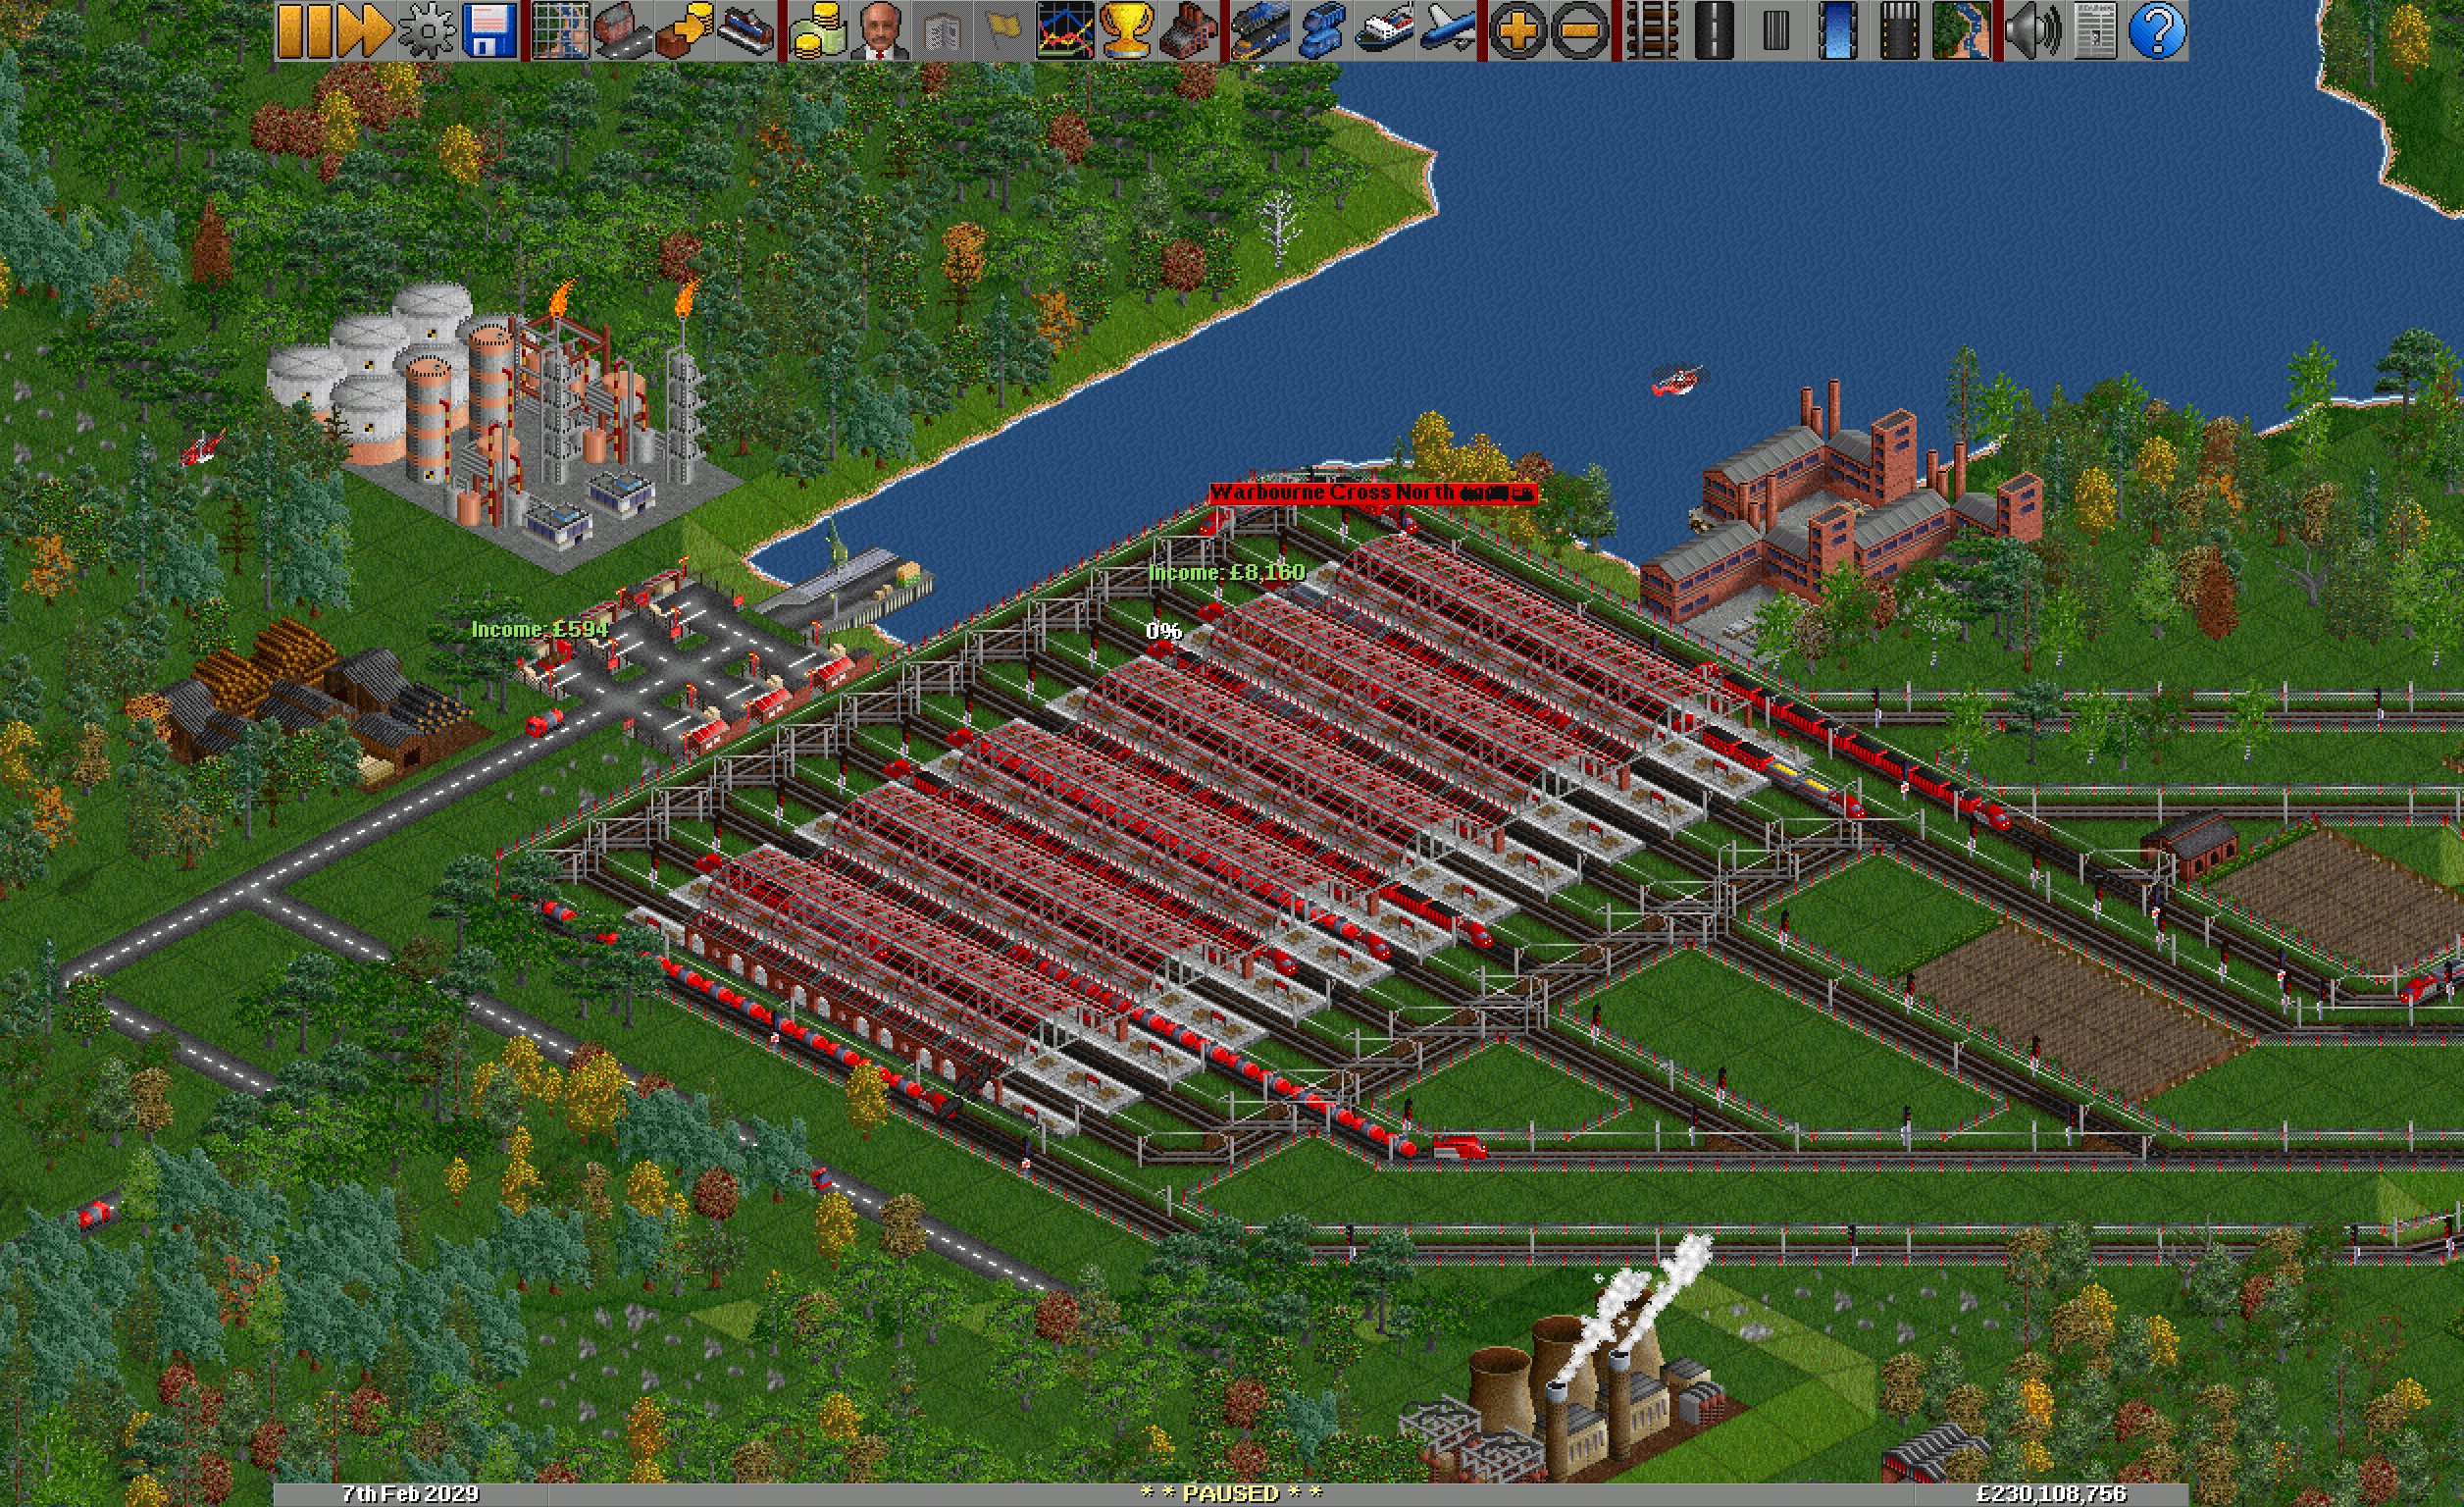
\includegraphics[width=\textwidth]{transport-tycoon-screenshot.png}
\caption{Screenshot of an OpenTTD game showing part of a transport network with multiple industries and mechanisms of transport. One of the trains has broken down, which not only prevents its cargo from reaching its destination, but it also prevents other trains from progressing along that track; OpenTTD has built-in ways of penalising non-robustness.}
\label{fig:network}
\end{figure}

OpenTTD is an open source business simulation game based on the 1990s game Transport Tycoon Deluxe. The aim of the game is to create a business that makes money from the transport of passengers and goods from one place to another, by constructing and using a network of road vehicles, trains, planes, or ships - also known as supply chains. An example of part of such a network can be seen in Figure \ref{fig:network}.

OpenTTD allows the implementation of so-called AIs, custom computer-based players that create their own supply chains to compete with human players. Over 50 such AIs have been created \cite{openttdAIs}. However, since OpenTTD is primarily a computer game rather than a tool for research, it is lacking in components for running reproducible experiments with such AIs and extracting data from them \cite{openttdNoHeadless}. The first aim of this project is to extend OpenTTD to allow such reproducible experiments.

The second aim of this project is to use OpenTTD and any extensions to construct an AI that allows the investigation of the links between robustness of such supply chains and other properties of the networks. While the focus of this project is OpenTTD, results could be compared with investigations of real-world supply chains, and so adds to the body of research of such supply chains, and so could be used to inform government and corporate policies.

\subsection{Problem Statement}

The first problem is the problem than OpenTTD is not suitable to run reproducible experiments. The work in this project is to change OpenTTD to make it possible to do so. For example, after initial investigation, it appears that OpenTTD does not support a mode to run the game at full speed without also running a graphical interface, and does not support the automated extraction of metrics or other details of the supply chains created.

The second problem is to answer the question \emph{In the game OpenTTD, what are properties of supply chains that are associated with resilience?}. This is a broad question - it will not be able to be answered conclusively in the time available. However, it should be able to be answered in some limited extent, for example by focusing on highly simplified worlds, a single transport mechanism, or simple supply chains of goods, or being robust to very limited events. Exactly what limitations will be applied will be chosen during the project.

\subsection{Research Hypothesis and Objectives}

Ideally, to make OpenTTD useful for reproducible research, any changes will be merged into its source code. And these changes will make it straightforward, so in a very low number of commands or configuration changes, to run experiments over a range of scenarios or AIs. Such steps can be measured - measuring the number of steps or decision points a researcher must take in order to run a set of experiments to produce some research. The ideal is a single step - a researcher running a single command, and results are output.

The second phase of the project has more of an open objective - to determine properties of supply chains in OpenTTD that offer robustness.

\subsection{Timeliness and Novelty}

While being based on a 1990s computer game, OpenTTD is actively developed and developed. For example, four releases have been made so far in 2023 \cite{openttdReleases}. The study of supply chain resilience is an active area of research, especially following the coronavirus (COVID-19) pandemic that started in 2020 and the 2021 Suez Canal obstruction by the container ship Ever Given. A systematic literature survey on research into supply chains and COVID-19 \cite{moosavi_supply_2022} showed that "resilience" was the top related keyword. However, it did not attempt to track changes over time. The results of a brief and informal analysis of published research indexed by Web of Science supply chain resilience is shown in Figure \ref{fig:supplychainresiliance} showing how supply chain research, and especially supply chain research mentioning with the COVID-19 pandemic, is not just active, but an increasing area of research.

\begin{figure}[h]
\centering
\begin{gnuplot}[terminal=cairolatex,terminaloptions={size 6,3}]
set tics font ",5"
set ylabel 'Number of publications'
set xlabel 'Year'
set style data histograms
set style histogram rowstacked
set style fill pattern border -1
set xtics nomirror
set ytics 100
set key invert
set key left top
set grid ytics
set xtics font ", 5"
set ytics font ", 5"
plot 'supply-chain-resiliance-research.dat' \
    using 2 t "  Without COVID-19", \
    '' using 3:xticlabels(1) t "With COVID-19" lc rgb '#999999'
\end{gnuplot}
\caption{The number of publications indexed by Web of Science matching the topic "supply chain resiliance" between 2014 and 2022, showing the split between publications with the topic COVID-19, and publications without. Data retrieved April 2023.}
\label{fig:supplychainresiliance}
\end{figure}

In terms of novelty, the first phase of the project solves the reported deficiency in OpenTTD - repeatedly running experiments with a parameterised AI for example is a manual process. In the second phase, OpenTTD does not appear to have been used in the study of resilient supply chains - as of April 2023 there no publications have been found indexed by Web of Science or Google Scholar linking OpenTTD with supply chain resilience.

\subsection{Significance}

The output of the first phase of the project, the headless mode of OpenTTD, is by itself valuable. It will others to reproduce any results from this project, and allow further research to be done using OpenTTD in a reproducible way. As can be seen by the Gantt chart in Figure \ref{fig:gantt}, almost half of the project time is dedicated to this. This is a deliberate choice to limit the risk of becoming part of the so-called reproducibility crisis \cite{baker_1500_2016}.

In terms of the second phase of the project, in terms of OpenTTD the direct answer is significant only in the  niche world of OpenTTD - its players and AI designers. However, the consequences of real-world supply chains can be serious, and addressing this has been described as an "urgent need" \cite{moosavi_supply_2022}. Thus any details that could be applicable to real-world supply chains could be significant.

\subsection{Feasibility}

The fact that OpenTTD is open source allow changes to be made. and the 50 existing AIs suggest its possible to make open AIs using a variety of algorithms. I'm an experienced software engineer with experience of working in unknown codebases, knowing several programming languages. Thus it should be feasible for me to make changes to the source code if necessary, and to write an AI in the available time. I'm also familiar with the pattern of creating my own tools and using them - which is what this project is. These facts makes this project feasible.

However, this project is ambitious and has unknowns. These facts introduce risks which are detailed in section \ref{riskassessment} along with their mitigations.

\subsection{Beneficiaries}

The first phase of the project should benefit researchers wanting to use OpenTTD for experiments. Code will be published so it is openly available, with clear instructions on how to use it in order to reproduce results. The ideal output of the first phase is to allow researches to reproduce any results in a single step, with any code changes merged into OpenTTD, so it will be ideally maintained for the lifetime of OpenTTD and more easily discoverable by other researchers. There have been previous modifications on forks of OpenTTD for research purposes \cite{shen_rtsenv_2011}, but I am unable to find the code of these changes, which makes the results in \cite{shen_rtsenv_2011} unreproducible. Every effort will be made to avoid a similar situation here.

The second phase of the project, the beneficiaries would be players and writers of OpenTTD AIs, researchers into supply chains, and potentially, anyone that can be affected by issues in supply chains.

It is expected that during the use of OpenTTD for research, improvements will be made to its headless mode from the first phase as deficiencies are found. Even if the output of the second phase isn't directly useful, it should improve the usefulness of the first.

\section{Background and Related Work}

OpenTTD has a challenging computational environment:

\begin{enumerate}

\item OpenTTD is based on an isometric two dimensional grid, the default size of which is 512 $\times$ 512 = 262144 tiles. Each tile has approximately 100 individual actions. Plus, there are actions that take multiple map tiles, for example building a station that can cover multiple tiles as can be seen in Figure \label{fig:network}. There are also actions that take place not directly on a tile, for example telling a vehicle to go to a particular station.

OpenTTD is a semi-real time game - is not possible to exhaustively consider all possible actions at all times.

\item Even if it were theoretically computationally feasible to consider all possible actions, OpenTTD limits the number of computations an AI can take in any given amount of time.

\item A field of play that is dynamic even if the AI chooses to take no action - you cannot perfectly apply any insights calculated from previous steps because the map may have changed.

\item Specifically enacting a plan, such as creating a rail network, takes time - the world may change during its construction. Decisions must be made whether to carry on, change, or abandon any construction.

\end{enumerate}

In existing AIs, these challenges been tackled using... PUT SOME IN

Describe some existing openttd AIs. Decision trees?

Things done in reproducibility, why not suitable

There do seem to have been a previous effort to make changes in OpenTTD in terms of reproducibility \cite{shen_rtsenv_2011}. However, as has already been discussed earlier, the specific details of these have not been found. Also, this project appears more focused on the scalability, memory, and CPU usage then any in-game properties.

Something to do with robust supply chains? What's been looked into there?

Specifically maybe similuating supply chains? How is robustness tested? At the very least - say this is to be discovered during the project

\section{Programme and Methodology}

This project will be done primarily in 2 phases that I'm calling Reproducibility and Resilience. In addition to these, there will be a short initial Preparation phase.

\begin{enumerate}
\addtocounter{enumi}{-1}
    \item \textbf{Preparation}

    There will be an initial short preparation phase of this project is make sure I have a dissertation template - will be virtually empty at the beginning, and that I can compile OpenTTD and make basic changes, and create and run a trivial AI. If I'm unable to do any of these steps, this must be discovered very early on in order to change the later plan.

    As discussed later in this proposal, it is deliberate to construct the dissertation at the beginning rather than a final writing up stage.
    
    \item \textbf{Reproducibility}

    The first main phase of the project focuses on making any required changes to OpenTTD in order to support reproducible research. This itself has two parts - a basic headless mode, and the construction of a naive AI developed using the headless mode. The purpose of the second part is to refine the headless mode in terms of usage and output, and to make sure that constructing an AI with certain properties is feasible in the time available.
    
    \item \textbf{Resilience}

    The second phase is to use the results of the previous phases to construct a parameterisable AI that can be used to investigate the relationship between properties of the networks it creates, and resiliance of those networks.

    The exact form of this AI will depend on discoveries during the previous phases. For example, rail networks are particular interesting due to their limited throughput, but are more difficult to construct.

    But still - speculate on the AI a bit now? Decision trees?
    
\end{enumerate}

In terms of methodology, this project will be undertaken in a highly iterative way - tight cycles of development and evaluation. There is suitable since this is an ambitious project with a number of unknowns. This will include maintaining a (mostly) ready to submit dissertation.

\subsection{Risk Assessment}
\label{riskassessment}

In terms of the first phase, to give maximum value to potential beneficiaries, any changes to OpenTTD would be merged into its codebase, and so maintained indefinitely. However, there is no guarantee of this. Although OpenTTD is actively maintained, PRs remain open from 2019 \cite{openTTDPRs}, and its maintainers are under no obligation to merge them or any PRs submitted as part of this project. However, there are migitations to this.

\begin{itemize}
    \item I'll submit changes as early as possible in the project.
    \item I'll submit changes that are as small as possible, and so more likely to be merged - from my own experience larger changes tend to be ignored for longer.
    \item I'll use what I submit as early on in the project as possible to make sure any changes are fit for at least one purpose.
    \item I'll continue to work as though changes will not be merged and maintain my own fork - the remainder of the project does not need to wait and will still output value without it.
\end{itemize}

Overall, the biggest risk is running out of time without any useful output - software projects are overdue 60\% of the time \cite{chaos2015}. From my own experience as a software engineer, projects where the engineer is not familiar with the domain have the highest risk of this. This is such a project - I am not familiar with the OpenTTD codebase, and to date have not written an OpenTTD AI.

To mitigate this risk, I leverage the fact that while the submission deadline is fixed, what is submitted by that deadline is not, allowing me to take a multi-scale agile/iterative approach to the project and adjust its aim as it progresses if necessary. Specifically:

\begin{itemize}
    \item Each phase/iteration is a de-facto feasibility study for the next phase.
    \item Each phase/iteration will result in value in terms of novelty, timeliness, and significance.
    \item Each phase/iteration will result in a reasonably complete project at all times.
\end{itemize}

To reduce the need to trade-off ambition against leaving time to write up, the iterations include the deliverable dissertation itself. The dissertation will be started at the beginning of the project rather than the end, and maintained as the project progresses. This is referred to as Continuous Delivery, and is often used when delivering web applications, for example \cite{chen_continuous_2015}. However, this approach has also been successfully used to include the deliver the written component of doctoral dissertations \cite{alipui_agile_nodate}, and so should be able to be applied here. I'm used to delivering working and useful software multiple times per day, and suspect that I can use similar workflows.

Figure \ref{fig:gantt} shows how this process can look in the style of a more traditional Gantt chart, and a summary of these risks are in Table \ref{fig:risks}.

\begin{table}[htbp]
    \begin{center}
        \begin{tabular}{|l|l|l|l|}
        \hline
        \textbf{Phases} & \textbf{Risk} & \textbf{Mitigations} & \textbf{Residual} \\
        \hline
        0, 1, 2 & Too time-consuming        & Earlier phase is feasibility study & Low \\
                &                           & Can expand on previous phases      & Low \\
                &                           & Re-plan                            & \\
        1       & Merges upstream take time & Initiate early                     & Low \\
                &                           & Make small, frequent changes       & Low \\
                &                           & Use what's submitted               & Low \\
                &                           & Maintain fork                      & \\
        2       & Non-reproducible results  & Create and use headless mode       & Low \\
                &                           & Maintain clear instructions        & Low \\
        \hline
        \end{tabular} 
    \end{center}
    \caption[Risks and mitigations]{Risks and mitigations}
    \label{fig:risks}
\end{table}

\subsection{Ethics}

All data will be generated during the project through simulations. Specifically, there will be no data collected from individuals.

However, there are actions that any AI could be deemed as unethical if applied to the real world. For example, it is possible that an AI destroys buildings while making the network. The headless mode can be extended to allow reporting on such actions.

\section{Evaluation}

The first phase of the project, making it easier for OpenTTD will be mostly qualitatively evaluated. Initially by myself, but ideally by OpenTTD maintainers who will decide whether to merge in any changes. There will also be an objective component - the number of manual steps required to be taken in order to reproduce research conducted with OpenTTD should be able to be counted before and after any changes.

The second phase of the project ??

\section{Expected Outcomes}

The outcome of the first phase of the project is that is will be easier to run reproducible experiments in OpenTTD. The second phase will use this output, refine it, and use it to help understanding the links between robustness of supply chains and other properties.

\section{Research Plan, Milestones and Deliverables}

The discussed plan of work can be seen summarised in Figure \ref{fig:gantt}, with the milestones in Table \ref{table:milestones}, and deliverables in Table \ref{table:deliverables}. The project has approximately 16 months available, on a part time basis.

\begin{figure}[htbp]
\begin{ganttchart}[
    vgrid,inline,
    x unit=1cm,
    time slot format=isodate-yearmonth,
    time slot unit=month,
    title height=1,
    group peaks height=0,
    group left shift=0,
    group right shift=0,
    group top shift=.7,
    bar height=.6
   ]{2023-05}{2024-08}
    \gantttitlecalendar{year, month=shortname} \\
    \ganttgroup{0 - Prep.}{2023-05}{2023-06} \\
    \ganttbar[name=dissertation, bar label font=\footnotesize]{Dissertation}{2023-05}{2023-06} \\
    \ganttbar[name=compile, bar label font=\footnotesize]{Compilation}{2023-05}{2023-06} \\
    \ganttgroup{1 - Reproducibility}{2023-07}{2023-12} \\
    \ganttgroup[group height=.1]{Headless mode}{2023-07}{2023-09} \\
    \ganttbar[name=i1]{1}{2023-07}{2023-07} \ganttlink[link mid=.166666]{compile}{i1} 
 \ganttlink[link mid=.375]{dissertation}{i1} \\
    \ganttbar[name=i2]{2}{2023-08}{2023-08} \ganttlink{i1}{i2} \\
    \ganttbar[name=i3]{3}{2023-09}{2023-09} \ganttlink{i2}{i3}  \\
    \ganttgroup[group height=.1]{Naive AI}{2023-10}{2023-12} \\
    \ganttbar[name=i4]{4}{2023-10}{2023-10} \ganttlink[link mid=.25]{i3}{i4} \\
    \ganttbar[name=i5]{5}{2023-11}{2023-11} \ganttlink{i4}{i5}   \\
    \ganttbar[name=i6]{6}{2023-12}{2023-12} \ganttlink{i5}{i6}   \\  
    \ganttgroup{2 - Resilience}{2024-01}{2024-08} \\
    \ganttgroup[group height=.1]{Parameterisable AI}{2024-01}{2024-08} \\
    \ganttbar[name=i7]{7}{2024-01}{2024-01} \ganttlink[link mid=.166666]{i6}{i7}  \\
    \ganttbar[name=i8]{8}{2024-02}{2024-02} \ganttlink{i7}{i8}  \\
    \ganttbar[name=i9]{9}{2024-03}{2024-03} \ganttlink{i8}{i9}  \\
    \ganttbar[name=i10]{10}{2024-04}{2024-04} \ganttlink{i9}{i10}  \\
    \ganttbar[name=i11]{11}{2024-05}{2024-05} \ganttlink{i10}{i11}  \\
    \ganttbar[name=i12]{12}{2024-06}{2024-06} \ganttlink{i11}{i12}  \\
    \ganttbar[name=i13]{13}{2024-07}{2024-07} \ganttlink{i12}{i13}  \\
    \ganttbar[name=i14]{14}{2024-08}{2024-08} \ganttlink{i13}{i14}
\end{ganttchart}
\caption[Project Gantt chart]{Gantt Chart of the activities defined for this project. This project will be undertaken on a part time basis and in a highly iterative way. Each iteration will contain reading, development, evaluation, and writing up. Each will result in complete project, albeit with limited scope.}
\label{fig:gantt}
\end{figure}

\begin{table}[htbp]
    \begin{center}
        \begin{tabular}{|S[table-format=2.0]|l|}
        \hline
    \textbf{Month} & \textbf{Milestone} \\
        \hline
        2 & Basic dissertation extended with the project \\
        2 & Can compile and make changes to OpenTTD \\
        5 & Headless mode created \\
        8 & Naive AI created along with refinements to headless mode \\
        16 & Complex AI created and used to investigate resilience \\
        \hline
        \end{tabular} 
    \end{center}
    \caption[Project milestones]{Project milestones}
    \label{table:milestones}
\end{table}
\begin{table}[htbp]
    \vspace{0.5cm}
    \begin{center}
        \begin{tabular}{|S[table-format=2.0]|l|}
        \hline
        \textbf{Month} & \textbf{Deliverable} \\
        \hline
        2 & Initial Dissertation \\
        5 & Initial headless mode \\
        8 & Naive AI as example of using headless mode \\
        16 & Parameterisable AI to investigate resilience \\
        16 & Final dissertation \\
        \hline
        \end{tabular} 
    \end{center}
    \caption[Project deliverables]{Project deliverables}
    \label{table:deliverables}
\end{table}


%                Now build the reference list
\bibliographystyle{unsrt}   % The reference style
%                This is plain and unsorted, so in the order
%                they appear in the document.

{\small
\bibliography{main}       % bib file(s).
}
\end{document}

